% Created 2019-08-05 Mon 18:33
% Intended LaTeX compiler: pdflatex
\documentclass[11pt]{article}
\usepackage[a4paper, margin=1in]{geometry}

\usepackage[vietnamese]{babel}
\usepackage[T1]{fontenc}
\usepackage{graphicx}
\usepackage{grffile}
\usepackage{longtable}
\usepackage{wrapfig}
\usepackage{rotating}
\usepackage[normalem]{ulem}
\usepackage{amsmath}
\usepackage{textcomp}
\usepackage{amssymb}
\usepackage{capt-of}
\usepackage{hyperref}
\usepackage{amsthm}
\usepackage{amsmath,amscd,amssymb,mathtools}
\usepackage{tikz-cd}
\usepackage{svg}
\usepackage[all]{xy}
\usepackage{pgfplots}
\newtheorem{remark}{Remark}
\newtheorem{theorem}{Theorem}
\newtheorem{lemma}[theorem]{Lemma}
\newtheorem{corollary}{Corollary}[theorem]
\newtheorem{conjecture}[theorem]{Conjecture}
\newtheorem{proposition}{Proposition}[theorem]
\newtheorem{problem}{Problem}
\newtheorem{exampl}{Example}
\newtheorem{definition}{Definition}
\newtheorem{propdef}[definition]{Proposition-Definition}
\newtheorem{fact}{Fact}
\newtheorem{assertion}{Assertion}
\newcommand{\re}{\mathop{\rm Re}\nolimits}
\newcommand{\im}{\mathop{\rm Im}\nolimits}
\newcommand{\coker}{\mathop{\rm coker}\nolimits}
\newcommand{\supp}{\mathop{\rm supp}\nolimits}
\newcommand{\ord}{\mathop{\rm ord}\nolimits}
\newcommand{\Spec}{\mathop{\rm Spec}\nolimits}
\newcommand{\vol}{\mathop{\rm vol}\nolimits}
\newcommand*{\transp}[2][-3mu]{\ensuremath{\mskip1mu\prescript{\smash{\mathrm t\mkern#1}}{}{\mathstrut#2}}}
\newcommand{\sff}{\mathop{\rm I\*I}\nolimits}
\newcommand{\tr}{\mathop{\rm Tr}\nolimits}
\newcommand{\const}{\mathop{\rm const }\nolimits}
\newcommand{\lcm}{\mathop{\rm lcm}\nolimits}
\newcommand{\Ric}{\mathop{\rm Ric}\nolimits}
\newcommand{\Riem}{\mathop{\rm Riem}\nolimits}
\newcommand{\Enorm}{\mathop{\mathcal{E}_{\rm norm}}\nolimits}
\newcommand{\Anorm}{\mathop{\mathcal{A}_{\rm norm}}\nolimits}
\newcommand{\Cl}{\mathop{\rm Cl }\nolimits}
\newcommand{\Spin}{\mathop{\rm Spin}\nolimits}
\newcommand{\Pin}{\mathop{\rm Pin}\nolimits}
\newcommand{\Hom}{\mathop{\rm Hom}\nolimits}
\newcommand{\End}{\mathop{\rm End}\nolimits}
\newcommand\restr[2]{{% we make the whole thing an ordinary symbol
\left.\kern-\nulldelimiterspace % automatically resize the bar with \right
#1 % the function
\vphantom{\big|} % pretend it's a little taller at normal size
\right|_{#2} % this is the delimiter
}}
\author{Bài tập Đại số tuyến tính đề nghị bởi Mạnh Tiến\footnote{Cựu sinh viên khoá 2010-2014.}}
\title{Giải thích một video của 3Blue1Brown bằng phép nhân ma trận}
\hypersetup{
 pdfauthor={},
 pdftitle={},
 pdfkeywords={},
 pdfsubject={},
 pdfcreator={Emacs 26.2 (Org mode 9.0.5)}, 
 pdflang={English}}
\begin{document}

\maketitle
\section*{Giới thiệu}
\label{sec:orgc6dd89a}
Trong một video trên kênh YouTube 3Blue1Brown (\emph{The most unexpected answer to a counting puzzle}, taị
\url{https://www.youtube.com/watch?v=HEfHFsfGXjs}) được chia sẻ rất nhiều trong thời gian gần
đây, Grant Sanderson đã giới thiệu bài toán sau của Gregory
Galperin về sự va chạm của 2 hình hộp như hình dưới đây, trong đó hộp bên trái có khối
lượng bằng 1 và hộp bên phải có khối lượng là \(m \geq 1\).
\begin{center}
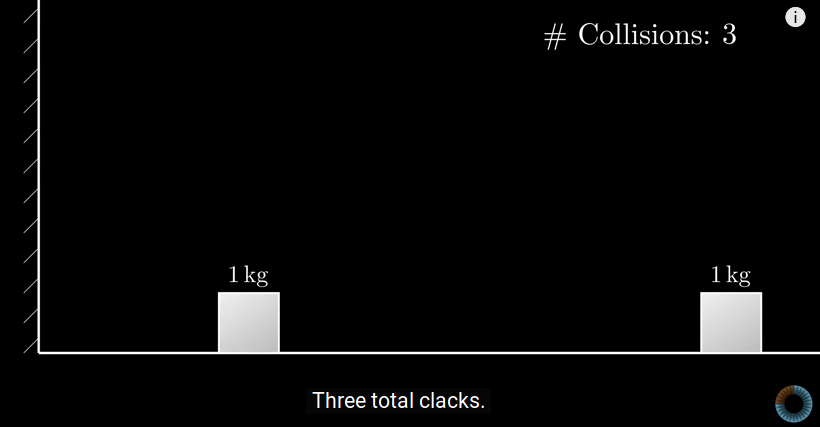
\includegraphics[width=.9\linewidth]{../img/3B1B-1.png}
\end{center}

Ở thời điểm bắt đầu, hộp bên phải chuyển động thẳng đều về phía tường (bên trái) và hộp trái đứng yên. Hai hộp
có thể va chạm với nhau và với tường. Giả sử không có ma sát và các va chạm đều
là đàn hồi (động lượng và năng lượng được bảo toàn), ta muốn đếm tổng số va chạm (hộp-hộp và
hộp-tường), chẳng hạn trong trường hợp khối lượng hai vật bằng nhau (\(m=1\)) có tổng
cộng 3 va chạm: hộp phải với hộp trái (sau đó hộp phải đứng yên), hộp trái với tường, và
hộp trái với hộp phải (sau đó hộp trái đứng yên). Trong trường hợp \(m=100\), tổng số va chạm
là 31 và nếu \(m=10000\), là 314. Grant Sanderson chỉ ra rằng nếu \(m\) là một lũy thừa của 100, giả sử \(100^k\) thì
số va chạm là \(k\) chữ số đầu tiên của số \(\pi\).

Youtuber này cho rằng thực hiện thí nghiệm này và đếm số va chạm là cách tính số \(\pi\)
đẹp nhất nhưng cũng kém hiệu quả nhất, so sánh khối lượng \(m\) cần thiết để
tính chính xác 20 chữ số thập phân của \(\pi\) với khối lượng một lỗ đen. Anh dành một
tuần để khán giả của mình suy nghĩ vì sao số \(\pi\) lại xuất hiện trong một bài toán va chạm đàn hồi.

Qua bài tập
sau, ta sẽ thấy đường tròn (hay số \(\pi\)) xuất hiện một cách tự nhiên qua góc argument của
giá trị riêng (phức) của một ma trận 2x2. Sử dụng một số
tính toán cơ bản được học trong môn đại số tuyến tính, ta sẽ chứng minh tổng số va chạm là
\[
N = \left \lfloor \frac{2\pi}{\arccos(\frac{m-1}{m+1})}\right\rfloor \text{ khi } m\geq 2
\]

Với \(m\) lớn, dùng khai triển Taylor \(\arccos(1 - 2\epsilon) = 2\sqrt{\epsilon} +
O(\epsilon^{3/2})\) ta có 
\[ 
\frac{2\pi}{\arccos(\frac{m-1}{m+1})} = \frac{2\pi}{2(m+1)^{-1/2} + O((m+1)^{-3/2})}=
\pi\sqrt{m+1} + O(\frac{1}{\sqrt{m+1}})  
\]
Do đó khi \(m=100^k\) thì \(N = \pi .10^k\) là \(k\) chữ số đầu tiên của \(\pi\).

\section*{Mô hình hoá}
\label{sec:org93c7835}
\subsection*{Va chạm giữa 2 hộp}
\label{sec:orgf5375ad}

Chọn chiều dương từ trái sang phải và gọi \(a,b\) lần lượt là vận tốc của hộp phải và
hộp trái trước khi va chạm, và \(a', b'\) là vận tốc ngay sau khi 2 hộp chạm nhau, định luật bảo toàn động lượng và
năng lượng (Sách giáo khoa Vật Lý lớp 10) nói rằng
\begin{equation*}
 \begin{cases}
\frac{1}{2}ma'^2 + \frac{1}{2}b'^2 = \frac{1}{2}ma^2 + \frac{1}{2}b^2,  \\
ma' + b' = ma + b
 \end{cases}
\end{equation*}
Viết lại phương trình thứ nhất thành \(\frac{1}{2}m(a' - a)(a'+a) =
\frac{1}{2}(b-b')(b+b')\) và thế \(m(a'-a) = b-b'\) (phương trình thứ 2)
ta có hệ phương trình
\begin{equation}
\label{eq:bb}
 \begin{cases}
a'-b' = a-b,  \\
ma' + b' = ma + b
 \end{cases}
\end{equation}


\paragraph{Câu 1.}
\label{sec:orgdba3652}
Dùng phép khử Gauss để tính \(a', b'\) theo \(a, b\) từ hệ phương trình
\eqref{eq:bb}. Viết lại dưới dạng phép nhân ma trận \(\begin{bmatrix} a'
\\ b' \end{bmatrix} = A_m  \begin{bmatrix} a
\\ b \end{bmatrix}\) với \(A_m\) là một ma trận 2x2 có các hệ số phụ thuộc vào \(m\). Tính \(A_m\).
\begin{proof}[Đáp án.]
\[
A_m =  \begin{bmatrix} \frac{m-1}{m+1} & \frac{2}{m+1}\\ \frac{2m}{m+1} &
\frac{1-m}{1+m} \end{bmatrix}
\]
\end{proof}


\subsection*{Va chạm với tường}
\label{sec:orga9110e9}
Vector vận tốc của hộp bên trái đổi chiều khi va chạm với tường. Nếu gọi \(a,b\) lần lượt là
vận tốc của hộp phải và hộp trái trước khi hộp trái chạm tường
và \(a', b'\) là vận tốc ngay sau khi chạm, ta có 
\begin{equation*}
\begin{bmatrix} a' \\ b'  \end{bmatrix} 
= B  \begin{bmatrix} a \\ b \end{bmatrix}
\text{ với } B = \begin{bmatrix}1 & 0 \\ 0 & -1 \end{bmatrix}
\end{equation*}


\subsection*{Điều kiện dừng}
\label{sec:orgd0dc201}
Vận tốc 2 hộp ban đầu được biểu diễn bởi vector \(\begin{bmatrix} a_0\\b_0 \end{bmatrix}
:= \begin{bmatrix} -1\\0 \end{bmatrix}\) và vận tốc sau \(n\) lần va chạm biểu diễn bởi
vector
\begin{equation*}
 \begin{bmatrix} a_n\\b_n \end{bmatrix} = \dots B A_m B A_m \begin{bmatrix} a_0\\b_0 \end{bmatrix}
\end{equation*}
cho bởi phép nhân bên trái xem kẽ với các ma trận \(A_m\) và \(B\), kết thúc bằng \(B\) nếu \(n\) chẵn và \(A_m\) nếu \(n\) lẻ.

Sẽ không còn va chạm khi và chỉ khi vận tốc cả 2 hộp đều dương và hộp bên phải đi nhanh
hơn hộp bên trái, nói cách khác là khi \(a_n\geq b_n\geq 0\). Bài toán được mô hình hoá
thành.

\paragraph*{Bài toán.}
\label{sec:org8b375c5}
Tìm số tự nhiên \(n\) nhỏ nhất sao cho \(a_n\geq b_n \geq 0\).

Nhận thấy rằng để tính \(a_n, b_n\), ta chỉ cần tính được lũy thừa của ma trận \(C :=A_m B\)

\paragraph{Câu 2.}
\label{sec:org7a31879}
Tính ma trận \(C := A_m B\). Tìm vết và định thức của \(C\). Bạn có nhận xét gì về 2
giá trị riêng của \(C\). 


\begin{proof}[Đáp án.]
\[
 C = \begin{bmatrix} \frac{m-1}{m+1} & \frac{-2}{m+1}\\ \frac{2m}{m+1} &
 \frac{m-1}{m+1} \end{bmatrix},\quad \tr(C) = 2\frac{m-1}{m+1},\quad \det C = 1
\]
\emph{Nhận xét.} Hai giá trị riêng của \(C\) là 2 số phức liên hợp có module 1, do đó được biểu diễn bởi
 một góc \(\theta\). Đây là lý do số
 \(\pi\) xuất hiện trong kết quả đếm. Dựa vào phần thực của chúng, ta thấy \(\theta =
 \arccos(\frac{m-1}{m+1})\) là góc đã nhắc đến trong đầu bài.
\end{proof}

\section*{Đơn giản hoá tính toán.}
\label{sec:org59250a0}
Nhận xét rằng \(\begin{bmatrix} a_0\\b_0 \end{bmatrix} = B\begin{bmatrix} a_0\\b_0
\end{bmatrix}\), ta viết lại
\[
 \begin{bmatrix} a_n\\b_n \end{bmatrix} = \dots B A_m B A_m B \begin{bmatrix} a_0\\b_0
\end{bmatrix} = \begin{cases}
B C^k	\begin{bmatrix} a_0\\b_0
\end{bmatrix}	,  & \text{khi $ n = 2k$} \\
C^k \begin{bmatrix} a_0\\b_0
\end{bmatrix}		, & \text{khi $n = 2k - 1$}
		\end{cases}
\]
trong đó \(C = A_m B\) là ma trận ở câu 2.

Một cách để tính \(C^k\) là chéo hoá ma trận \(C\), vì khi \(C = P^{-1} D P\) với \(D = \begin{bmatrix} \lambda_1 & 0\\ 0 &
\lambda_2 \end{bmatrix}\) là một ma trận chéo thì \(C^k = P^{-1}D^k P\) với \(D^k = \begin{bmatrix} \lambda_1^k & 0\\ 0 &
\lambda_2^k \end{bmatrix}\).

\paragraph{Câu 3.}
\label{sec:org7c9b1d6}
Ma trận \(C\) có chéo hoá được trên \(\mathbb{C}\) không? Lưu ý: Bạn không cần chéo hóa ma trận
\(C\) để trả lời.
\begin{proof}[Đáp án.]
Có. Nhắc lại rằng một ma trận vuông bậc \(k\) chéo hoá được khi và chỉ khi tổng số chiều
cuả các không gian riêng bằng \(k\). Do 2 giá trị riêng cuả \(C\) khác nhau nên \(C\) có 2 không gian riêng, số chiều của mỗi
không gian ít nhất là 1 nên tổng số chiều đúng bằng 2.
\end{proof}


Sau đây ta sẽ tính luỹ thừa của ma trận \(C\) mà không chéo hoá.

\paragraph{Câu 4.}
\label{sec:org931b7ff}
Tính đa thức tối tiểu \(Q(X)\) của ma trận \(C\).
\begin{proof}[Đáp án.]
Nhắc lại rằng đa thức tối tiểu là ước của đa thức đặc trưng của \(C\), i.e. \(X^2 - 2 \frac{m-1}{m+1} X + 1 = 0\). Do 2 giá trị
riêng của \(C\) khác nhau nên đa thức tối tiểu cũng là đa thức đặc trưng.
\end{proof}

Ta sẽ tính \(C^k\) bằng cách thực hiện phép chia đa thức \(X^k\) cho \(Q(X)\):
\begin{equation}
\label{eq:min-pol}
 X^k = P_k(X)Q(X) + u_k X + v_k, \quad P_k\in \mathbb{R}[X], \quad u_k, v_k\in \mathbb{R}
\end{equation}
Do đa thức \(Q\) triệt tiêu \(C\), ta có thể tính \(C^k = u_k C + v_k\) nếu biết hai
số thực \(u_k\) và \(v_k\). 

Gọi \(\lambda\) và \(\bar\lambda = \lambda^{-1}\) là hai
giá trị riêng của \(C\).


\paragraph{Câu 5.}
\label{sec:orgbe50be4}
Chứng minh rằng \(u_k = \frac{\lambda^{2k} - 1}{\lambda^{k-1}(\lambda^2-1)} =
\lambda^{-(k-1)} + \lambda^{-(k-1) + 2} + \dots + \lambda^{k-1}\) và \(-v_k
=  \frac{\lambda^{2(k-1) - 1}}{\lambda^{k-2} (\lambda^2-1)} = \lambda^{-(k-2)} +
\lambda^{-(k-2) + 2} + \dots + \lambda^{k-2}\).
\begin{proof}[Đáp án.]
Thế \(X\) bởi \(\lambda\) và \(\bar \lambda\) vào
\eqref{eq:min-pol}, lưu ý rằng \(Q(X)=0\), ta có hệ phương trình
\begin{equation*}
 \begin{cases}
u_k\lambda + v_k = \lambda^k   \\
u_k\bar \lambda + v_k = \bar\lambda^k 
 \end{cases}
\end{equation*}
Sau đó giải hệ phương trình này để tính \(u_k, v_k\).
\end{proof}


\paragraph{Câu 6.}
\label{sec:org0f2208f}
Tính \(\begin{bmatrix} a_{2k-1}\\b_{2k-1} \end{bmatrix} = C^k \begin{bmatrix} -1\\0
\end{bmatrix}\) và \(\begin{bmatrix} a_{2k}\\b_{2k} \end{bmatrix} = BC^k \begin{bmatrix} -1\\0
\end{bmatrix}\) theo \(u_k, v_k\). Thay \(\frac{m-1}{m+1} = \frac{1}{2}(\lambda + \lambda^{-1})\)
và \(\frac{2m}{m+1} = \frac{1}{2}(\lambda + \lambda^{-1}) + 1\), chứng minh rằng \(a_{2k-1} - b_{2k-1} = u_k - v_k\) và \(b_{2k} - a_{2k} = u_k - v_k +\lambda^k + \lambda^{-k}\)
\begin{proof}[Đáp án.]
\begin{equation*}
 \begin{bmatrix} a_{2k-1}\\b_{2k-1} \end{bmatrix}   = \begin{bmatrix} -u_k.\frac{m-1}{m+1} -
v_k\\-u_k.\frac{2m}{m+1} \end{bmatrix}, \qquad \begin{bmatrix} a_{2k}\\b_{2k} \end{bmatrix}=  \begin{bmatrix} -u_k.\frac{m-1}{m+1} -
v_k\\u_k.\frac{2m}{m+1} \end{bmatrix}
\end{equation*}
Với \(b_{2k} - a_{2k}\), để ý rằng \(u_k\lambda^{\pm 1} = -v_k + \lambda^{\pm k}\).
\end{proof}

\section*{Trực quan hình học}
\label{sec:org735e1e5}

Viết \(\lambda = e^{i\theta}\) với \(\theta =
 \arccos(\frac{m-1}{m+1})\).  Với mọi \(k\geq 1\), đặt
\[
S^2_k:= \lambda^{-k} + \lambda^{-k+2} + \dots + \lambda^{k-2} + \lambda^k\quad \text{và}\quad S^1_k = \lambda^{-k} + \lambda^{-k+1} + \dots + \lambda^{k-1} + \lambda^k
\]


\paragraph{Câu 7.}
\label{sec:org8b3528c}
Chứng minh rằng \((a_{2k-1},b_{2k-1})\) thoả mãn điều kiện
dừng \(a_{2k-1}\geq b_{2k-1}\geq 0\) khi và chỉ khi \(S^1_{k-1} \geq 0\) và \(S^{2}_{k-1}\leq 0\). Chứng minh rằng \((a_{2k},b_{2k})\) thoả mãn điều kiện
dừng \(a_{2k}\geq b_{2k}\geq 0\) khi và chỉ khi \(S^1_{k} \leq 0\) và \(S^{2}_{k-1}\geq 0\).
\begin{proof}[Đáp án.]
Hiển nhiên khi viết lại \(u_k = S^2_{k-1}\), \(u_k-v_k = S^1_{k-1}\) và \(u_k-v_k +\lambda^k +\lambda^{-k} = S^1_{k}\).
\end{proof}

Xem \(S^2_k\) ( tương ứng \(S^1_k\)) là tổng của \(k+1\) (tương ứng \(2k+1\))
vector cách đều trên đường tròn đơn vị, mệnh đề sau là hiển nhiên về mặt trực quan và
được thừa nhận.

\paragraph*{Mệnh đề.}
\label{sec:org28d33d0}
Giả sử \(k\leq \left \lfloor \frac{\pi}{\theta} \right\rfloor\). Khi đó 
\begin{enumerate}
\item \(S^1_k \leq 0\) khi và chỉ khi cung tròn từ \(\lambda^k\) đến \(\lambda^{-k}\) nhỏ hơn hoặc bằng \(\theta\).
\item \(S^2_k \leq 0\) khi và chỉ khi cung tròn từ \(\lambda^k\) đến \(\lambda^{-k}\)
nhỏ hơn hoặc bằng \(2\theta\).
\end{enumerate}


\paragraph{Câu 8.}
\label{sec:orga1c47d8}
Dùng mệnh đề, chứng minh rằng với \(h =  \left \lfloor \frac{\pi}{\theta} \right\rfloor\) thì hoặc \((a_{2h}, b_{2h})\) hoặc \((a_{2h+1}, b_{2h+1})\) thoả điều kiện dừng,
còn các bộ \((a_i, b_i)\) với \(i < 2h\) không dừng. Từ đó suy ra \(N = \left \lfloor
\frac{2\pi}{\theta} \right \rfloor\).
\begin{proof}[Đáp án.]
Nếu cung từ \(\lambda^h\) đến -1 nhỏ hơn \(\frac{\theta}{2}\) thì \((a_{2h}, b_{2h})\) dừng, ngược lại thì \((a_{2h+1}, b_{2h+1})\) dừng.
\end{proof}

Một tuần sau video nói trên, Grant Sanderson đưa ra lời giải của anh tại
\url{https://www.youtube.com/watch?v=jsYwFizhncE} bằng một lập luận tương đối đơn giản. Kết quả của
anh là \(N = \left \lfloor \frac{\pi}{\phi} \right\rfloor\) với \(\phi = \arctan
\frac{1}{\sqrt{m}}\)

\paragraph{Câu 9 (Không tính điểm).}
\label{sec:org99e9f8f}
So sánh số va chạm \(N\) ở đầu bài vơí kết quả cuả Grant Sanderson.
\begin{proof}[Đáp án.]
\(\theta = 2\phi\).
\end{proof}

\end{document}
%%% Local Variables:
%%% mode: latex
%%% TeX-master: t
%%% End:
